\section{System Specifcation}
This section describes the specification of the new system.

\begin{figure}[H]
  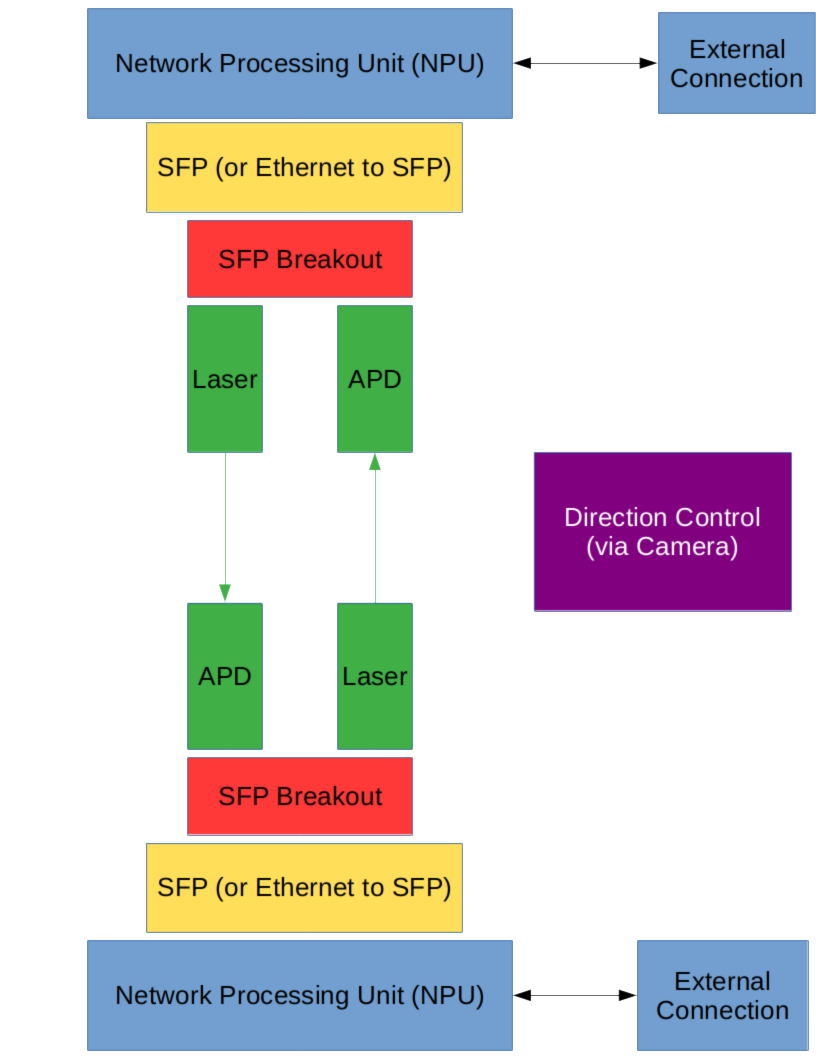
\includegraphics[width=0.8\textwidth]{system_design.png}
  \caption{System Design for high speed underwater network}
  \label{fig:system-design}
\end{figure}

\paragraph{\textbf{System Highlights}}
\begin{itemize}
\item{5V maximum}
\item{\ac{SFP}-based, using breakout board to transmitter and receiver}
\item{1 Gb/s data rate}
\item{Utilizing
	\url{https://mikrotik.com/product/RB922UAGS-5HPacD#fndtn-specifications}
	or similar for SFP}
\item{Laser - same as current. Needs to be able to transmit at 1 Ghz using
	\ac{OOK}}
\item{Receiver - same as current. Needs to receive a 1 Ghz \ac{OOK} signal}
\item{Tracking - done with camera. Current suggestion is to use PIXY 2
	\url{https://pixycam.com/pixy2/}.}
\item{Case - waterproof with a 180 degree underwater housing. E.g.
	\url{https://www.okorder.com/p/underwater-360-rotate-camera-for-rov-use_408066.html}}
\end{itemize}

We are going to build an \ac{SFP} based point to point system, as the
directionality of the lasers mean point to multi-point does not need to be
supported.

KORUZA has already shown that an Ethernet based approach can work, so we will
utilize this.

The system will support at least 1 Gb/s data rate, so it is fast enough
for most traffic (aside from uncompressed video streaming).
